\subsection{Lösungen der Dirac-Gleichung und der nicht relativistische Grenzfall}
Einheiten Konvention $\boxed{c=1=\hbar}$
\subsubsection{Ruhende Teilchen $\partial_t \psi = 0$}
\begin{eqnarray*}
i\partial_t \psi = m \beta \psi
\end{eqnarray*}
Die Dirac-Gleichung für ein räumlich unabhängiges Teilchen. Wir können 4 linear unabhängige Lösungen angeben, müssen jedoch die Zeitabhängigkeit beachten.
$$\psi(t) = \psi e^{-iEt}$$
\begin{alignat*}{4}
\psi_1^+ = \left( \begin{array}{c} 1\\0\\0\\0\end{array}\ri ) e^{-imt} \qquad\qquad \psi_2^+ \g  
\left . \left(\begin{array}{c} 0\\1\\0\\0\end{array}\ri ) e^{-imt} \ri \} E = m c^2\\
\psi_1^- = \left( \begin{array}{c} 0\\0\\1\\0\end{array}\ri ) e^{+imt} \qquad\qquad \psi_2^- \g  
\left . \left(\begin{array}{c} 0\\0\\0\\1\end{array}\ri ) e^{+imt} \ri \} E = -m c^2
\end{alignat*}
Jeweils zwei Lösungen mit \underline{positiver} und \underline{negativer} Energie!\\
\underline{Bedeutung?}
\begin{itemize}
\item 2 Lösungen mit positiver Energie entsprechen den {\bf inneren Freiheitsgraden}.\\
$\Longrightarrow$ Eigendrehimpuls = Spin.
\item Lösungen negativer Energie entsprechen Antiteilchen, die erst im Rahmen der Quantenfeldtheorie konsistent behandelt werden können.
\end{itemize}

\subsubsection{Ebene Wellen}
Wir suchen Lösungen der Klein-Gordon-Gleichung
\begin{eqnarray*} (\Box + m^2 ) \psi \g 0\\
\rightarrow - p^2+ m^2\g  0 \qquad \Rightarrow E^2 = m^2 + \vec p^2\\
\longrightarrow E \g \pm \sqrt{m^2+ \vec p^2}
\end{eqnarray*}
Seien $u_s$ und $v_s$ Spinoren, so lässt sich abhängig von der Energie schreiben:
\begin{alignat*}{4}
E &>& 0 \qquad \psi^+ (x) \g u_s(\vec p) e^{-ip x} = u_s(\vec p) e^{-ip_0t+i\vec p\vec x}\\
E &<& 0 \qquad \psi^- (x) \g\  v_s(\vec p) e^{ip x} =v_s (\vec p) e^{ip_0t-i\vec p\vec x}
\end{alignat*}
Hierbei ist $p_0 = \sqrt{m^2+ \vec p^2} > 0$. Die Spinoren erfüllen mit $i\slashed{\partial} \psi = \pm \slashed p \psi$ die Dirac-Gleichung:
\begin{eqnarray*}
\big ( \slashed p - m \big ) u_s(\vec p) \g 0\\
\big ( \slashed p + m \big ) v_s(\vec p) \g 0
\end{eqnarray*}
Benutze zur Berechnung:
\begin{eqnarray*}
\slashed p \slashed p \g p_{\mu}\gamma^{\mu} p_ \nu \gamma^\nu = p_\mu p_\nu \frac 1 2 \underbrace{\big\{\gamma^\mu,\gamma^\nu \big \}}_{2 g^{\mu \nu}}\\
\g p_\mu p_\nu g^{\mu\nu} = p_\mu p^\mu \overset * = m^2
\end{eqnarray*}
*) Das einzige Lorentzskalar, welches unter Transformationen konstant bleibt ist $m^2$.\\
Es gilt also:
\begin{eqnarray*}
\big (\slashed p - m \big )\big(\slashed p + m \big) \psi = \big ( \slashed p \slashed p - m^2 \big ) \psi = 0
\end{eqnarray*} 
D.h. ein Spinor $\psi' = \big ( \slashed p + m \big ) \psi$ erfüllt die Dirac-Gleichung, da 
\begin{eqnarray*}\big(\slashed p - m \big ) \psi' = \big ( \slashed p - m \big) \big(\slashed p + m\big )\psi =0\end{eqnarray*}
 für ein beliebiges $\psi$.\\
$\Longrightarrow$ Wir erhalten Lösungen z.B. indem wir $\big (\slashed p \pm m \big)$ auf die Basisvektoren 
\begin{eqnarray*} u_0 = \left ( \begin{array}{c} \chi_s\\0\end{array}\ri )\qquad
\text{mit }\chi_{\pm} = \left ( \begin{array}{c} 1\\0\end{array} \ri ),\left ( \begin{array}{c} 0\\1\end{array} \ri )
\end{eqnarray*} anwenden.
\begin{eqnarray*}
\big( \slashed p + m \big ) u_0 \g \big ( p^\mu \gamma_\mu + m \big ) u_0 = \left (\begin{array}{cc} (E+m){\mathds {1}}_2 & -\vec p\hat{\vec \sigma} \\ \vec p \hat{\vec \sigma}& (-E+m){\mathds 1}_2 \end{array}\ri) \cdot\left ( \begin{array}{c} \chi_s\\0\end{array}\ri) \\ \g \left( \begin{array}{c} (E+m)\chi_s \\\vec p\hat{\vec \sigma} \cdot \chi_s\end{array}\ri)\\
\vec p \vec \sigma \g p_x\sigma_x + p_y\sigma_x + p_z \sigma_z = \left ( \begin{array}{cc} p_z & p_x+ip_y\\p_x-ip_y&-p_z\end{array}\ri)\\
\text{analog}&{}& (\slashed p - m) \left( \begin{array}{c} \chi_s\\0 \end{array}\ri )
\end{eqnarray*}
$\longrightarrow$ vier linear unabhängige Lösungen (Normierung später).
\begin{eqnarray*}
\boxed{ u_s (\vec p) = \sqrt{\frac{E+m}{2m}} \left(\begin{array}{c} \chi_s\\ \frac{\vec p \hat{\vec \sigma}}{E+m} \chi_s\end{array}\ri )}\\
 \boxed{v_s (\vec p) = \sqrt{\frac{E+m}{2m}} \left(\begin{array}{c} \frac{\vec p \hat{\vec \sigma}}{E+m} \chi_s\\ \chi_s\end{array}\ri )}
\end{eqnarray*}
Die vollständigen Wellenfunktionen sind:
\begin{eqnarray*}
\psi^+ _{\vec p,s}(\vec r,t) \g u_s(\vec p)e^{i(\vec p\vec r-Et)} \qquad \text{mit }E = \sqrt{m^2+ \vec p^2}\\
\psi^- _{\vec p,s}(\vec r,t) \g v_s(\vec p)e^{i(-\vec p\vec r+Et)}
\end{eqnarray*}
Zum Beweis der Orthogonalität benötigen wir zunächst die Definition des Skalarprodukts im Spinorraum. Hierzu führen wir den adjungierten Spinor $\bar \psi = \psi^{\dagger} \gamma_0$ ein.
(vgl. hermitesch adjungiert: $\psi^{\dagger} = \psi^{T*}$.)\\
Damit gilt für die Dichte und den Strom:
\begin{eqnarray*} 
j^\mu \g c \Big ( \psi^\dagger \psi, \psi^\dagger \vec \alpha \psi\Big)\\
\g c \Big ( \bar \psi \gamma^0 \psi, \bar \psi \vec \gamma \psi \Big)\\
\g c \bar \psi\gamma^\mu \psi 
\end{eqnarray*}
Für die adjungierten Spinoren gilt:
\begin{eqnarray*} \bar u_s = u_s^\dagger \gamma_0 \g \sqrt{\frac {E+m}{2 m}}\Big(\chi^\dagger_s,\chi_s^\dagger \frac{\vec p\hat{\vec \sigma}}{E+m}\Big)\left(\begin{array}{cc}1&0\\0&-1\end{array}\ri)\\
\g\sqrt{\frac {E+m}{2 m}}\Big(\chi^\dagger_s,-\chi_s^\dagger \frac{\vec p\hat{\vec \sigma}}{E+m}\Big)\\
\bar v_s \g \sqrt{\frac {E+m}{2 m}}\Big(\chi^\dagger_s \frac{\vec p\hat{\vec \sigma}}{E+m},-\chi_s^\dagger\Big)\\
\bar u_s \cdot u_{s'} \g \frac {E+m}{2 m}\Big(\chi^\dagger_s \chi_{s'}-\chi_s^\dagger \left(\frac{\vec p\hat{\vec \sigma}}{E+m}\ri)^2\chi_{s'}\Big)
\end{eqnarray*}
Mit der Identität $(\vec p \hat{\vec \sigma})^2=\vec p^2$ vereinfachen, wir das
\begin{eqnarray*}
\rightarrow \bar u_su_{s'} \g \frac{E+m} {2m}\delta_{ss'} \Big(1 - \frac{\vec p^2}{(E+m)^2}\Big) = \delta_{ss'}\\
\bar u_sv_{s'} \g \frac{E+m}{2m} \Big( \chi_s^\dagger \frac{\vec p\hat{\vec \sigma}}{E+m}\chi_{s'} - \chi_s^\dagger \frac{\vec p\hat {\vec\sigma}}{E+m}\chi_s\Big)= 0\\
\Longrightarrow &{}& \boxed{\begin{array}{ll}\bar u_s u_{s'} = \delta_{ss'} &\bar v_s v_{s'} = -\delta_{ss'}\\\bar u_s v_{s'} = 0 & \bar v_s u_{s'} = 0 \end{array}}
\end{eqnarray*}
Die umrahmte Gleichung gilt unabhängig vom Bezugssystem, da die rechten Seiten nicht vom Impuls abhängen.\\
Wir berechnen die Dichte $\rho = \frac{j^0}c = \bar \psi \gamma^0 \psi$ mit Hilfe von
\begin{eqnarray*}
\frac{\slashed p}mu_s = u_s \qquad \big((\slashed p - m) u_s = 0 \big)
\end{eqnarray*}
Es gilt nun:
\begin{eqnarray*}
\bar \psi_s^+ \gamma_0\psi_s^+ \g \bar\psi_s^+ \underbrace{\frac{\slashed p \gamma_0+\gamma_0\slashed p}{2m}}_{\frac 1 {2m}\big\{\slashed p , \gamma_0\big\} = \frac 1{2m}2p_0=\frac E m} \psi^+_s \\ \g \frac E m\\
\bar \psi^-_s\gamma_0\psi^-_s &\overset{-\frac{\slashed p} m v_s = v_s}=&\bar \psi^-_s \frac{\slashed p \gamma_0-\gamma_0\slashed p}{2m}\psi_s^- =-\frac E m\bar v_s v_s \\ \g \frac E m
\end{eqnarray*}
$\longrightarrow$ Die Dichten sind positiv für alle Lösungen, aber sie sind kein Lorentzskalar (aufgrund der Längenkontraktion unter Lorentztransformationen ist das verständlich). Der faktor $\frac E m$ kann auch geschrieben werden als:
\begin{eqnarray*}
\frac E m = \frac {\frac E {m_0}} {\sqrt{1 - \frac {v^2}{c^2}}} = \gamma \frac E {m_0}
\end{eqnarray*}
und kompensiert die Längenkontraktion des Volumeneleents $\frac{d^3x}  \gamma$.\\
\\
Berechnung der Stromdichte.
\begin{eqnarray*}
\vec j \g c \bar \psi\vec \gamma \psi \qquad\qquad \psi = \left \{ \begin{array}{ll} u_{\vec p,s}&e^{i(\vec p\vec r-Et)}\\v_{\vec p,s}&e^{-i(\vec p\vec r-Et)}\end{array}\ri.\\
\bar u_{\vec p,s}\vec \gamma u _{\vec p,s}\g \Big(\chi^\dagger_{s}, -\chi_s^\dagger \frac{\vec p\hat{\vec\sigma}}{E+m}\Big) \left(\begin{array}{cc}0 &\vec \sigma\\-\vec \sigma&0\end{array}\ri )\left(\begin{array}{c} \chi_s\\ \frac{\vec p\hat{\vec \sigma}}{E+m}\chi_s\end{array}\ri ) \frac{E+m}{2m}\\
\g \chi^\dagger_s \Big(\hat{\vec\sigma}(\vec p \hat{\vec \sigma}) + (\vec p \hat{\vec \sigma})\hat{\vec \sigma}\Big) \chi_s \frac1 {2m}\qquad \text{mit }\big\{\sigma_i,p_j\sigma_j\big\} = 2p_i\\
\g \frac{\vec p}m\\
\text{Ebenso gilt}&{}& \bar v_{\vec p,s}\vec \gamma v_{\vec p,s} = \frac{\vec p}m
\end{eqnarray*}
$\longrightarrow$ Die Stromdichte zeigt in $\vec p$-Richtung für $\psi^+$ und $\psi^-$.\\
$\longrightarrow$ Beachte $\psi^+\sim e^{i\vec p\vec r}$ aber $\psi^- \sim e^{-i\vec p\vec r}$bewegt sich in umgekehrter Richtung

\subsubsection{Ankopplung des elektromagnetischen Feldes}
Wir wenden das Prinzip der minimalen Kopplung an und ersetzen den Impulsoperator gemäß:
\begin{eqnarray*}
\vec p \rightarrow \vec p - q \vec A = \vec \Pi
\end{eqnarray*}
Weiter addieren wir die potentielle Energie zum Hamiltonoperator
\begin{eqnarray*} \wh \ham \rightarrow \wh \ham + q \Phi\end{eqnarray*}
Zusammenfassen für die restliche Rechnung:
\begin{eqnarray*}
p^\mu &\rightarrow& p^\mu - q A^\mu \qquad A^\mu = \Big ( \Phi , \vec A \Big)\\
i\hbar \partial ^\mu &\rightarrow& i \hbar \partial^\mu - q A^\mu
\end{eqnarray*}
Einsetzen in die Dirac-Gleichung ergibt:
\begin{eqnarray*}\nonumber
\left(i\hbar \partial _ \mu \gamma^\mu - q A_\mu\gamma^\mu - m c\ri) \psi = 0\\\label{eq:6}
\boxed{\left(i\slashed \partial - q \slashed A - m c\ri) = 0}
\end{eqnarray*}
Die Gleichung (\ref{eq:6}) ist die Dirac-Gleichung im elektromagnetischem Feld (in eichinvarianter Form). 

\subsubsection{Nicht-relativistischer Grenzfall, Pauli-Gleichung}
Ebene Welle für $\left|\vec p\ri|/m \ll c\quad (mc^2\gg c \left|\vec p\ri|)$
\begin{eqnarray*}
u_s(\vec p) = \sqrt{\frac{E+m c^2}{2mc^2}} \cdot \left ( \begin{array} c \chi_s \\ \frac{\vec p \hat {\vec \sigma}}{E + m c^2}\chi_s\end{array}\ri)\overset{E\rightarrow m c^2}{\longrightarrow} \left ( \begin{array}{c}\chi_s \\ \frac{\vec p\hat{\vec\sigma}}{2 m c^2}\chi_s\end{array}\ri)
\end{eqnarray*}
Die unteren Komponenten sind um einen Faktor
\begin{eqnarray*}
\frac{\left|\vec p\ri|}{m c} \approx \frac v c 
\end{eqnarray*}
kleiner.
Die Dirac Gleichung in der hamiltonschen Schreibweise:
\begin{eqnarray*}
i\hbar \partial _ t\psi = \left(\vec \Lr \vec Pi \vec \alpha + q \Phi + m \beta\ri ) \psi
\end{eqnarray*}
Ansatz:
\begin{eqnarray*}
\underline \psi = \left (\begin{array} {c} \tilde{\phi}\\ \tilde \chi\end{array}\ri) \qquad \quad \begin{array}{ccc} \tilde \phi & : &\text{,,große Komponente''}\\\tilde \chi & : &\text{,,kleine Komponente''}\end{array}
\end{eqnarray*}
$\rightarrow$ Separieren die schnellen zeitlichen Oszillationen ab (verursacht durch die dominante Energie $mc^2$).
\begin{eqnarray*}\nonumber
\left(\begin{array} c \tilde \phi \\ \tilde \chi \end{array}\ri ) \g e^{-imt} \left(\begin{array}{c}\phi\\ \chi \end{array}\ri)\\\label{eq:7}
\Longrightarrow i\hbar\partial_t\left(\begin{array} c \phi \\ \chi \end{array}\ri) \g \vec \Pi \vec \sigma \left(\begin{array}c \chi\\\phi\end{array}\ri) + q \Phi \left(\begin{array}c \phi\\ \chi\end{array}\ri) - 2 m \left(\begin{array}c 0 \\ \chi\end{array}\ri)
\end{eqnarray*}
$\chi$ ist um $\frac v c \approx  \frac{\left|\vec \Pi\ri|}{m c}$ kleiner als $\phi$, d.h. wir können $\dot \chi$ und $e \Phi \chi$ vernachlässigen.\\
Die Gleichung für $\chi$ ist dann
\begin{eqnarray*}
\chi = \frac{\vec\Pi\hat{\vec \sigma}}{2mc}\phi.
\end{eqnarray*}
Einsetzten in die Gleichung (\ref{eq:7}) für die obere Komponente ergibt:
\begin{eqnarray*}
i\hbar \partial_t \phi  = \left[ \frac{1}{2m} \left(\vec \Pi \hat{\vec\sigma}\ri)^2 + e \Phi \ri] \phi
\end{eqnarray*}
Auswerten mit der Identität:
\begin{eqnarray*}
(\vec a \hat{\vec \sigma})(\vec b \hat{\vec \sigma}) \g \vec a\vec b + \hat{\vec \sigma}(\vec a \times \vec b)\qquad \text{mit }[a,\sigma] = 0 = [b, \sigma]\\
\text{d.h.} (\vec \Pi\hat{\vec \sigma})^2 \g \vec \Pi^2 + i \hat{\vec \sigma}(\vec \Pi\times\vec\Pi)
\end{eqnarray*}
Aus Kapitel I.5.3 folgt für $\vec \Pi$
\begin{eqnarray*}
&{}&\vec \Pi = m \vec v_{\text{op}} = -i\hbar \vec \nabla - q \vec A\\
\rightarrow &{}& \vec \Pi \times \vec \Pi = i q \hbar \vec B
\end{eqnarray*}
Hiermit ergibt sich die {\bf Pauli-Gleichung} zu:
\begin{eqnarray*} \boxed{
i\hbar \partial_t \phi= \left[\frac 1 {2m} \left( \vec p - q \vec A\ri)^2 - \frac{\hbar }{2m}\hat{\vec\sigma}\vec B + q \Phi\ri ]\phi}
\end{eqnarray*}
Im konstanten Magnetfeld $\vec B = \rot \vec A$
\begin{eqnarray*} \vec A = \frac 1 2\vec B \times \vec r\qquad\qquad \divergenz  \vec A = 0
\end{eqnarray*} 
Für die Drehimpulsoperatoren gilt:
\begin{eqnarray*}
\vec L = \vec r \times p \qquad \qquad \vec S = \frac \hbar 2 \hat{\vec \sigma}
\end{eqnarray*}
Somit erhalten wir
\begin{eqnarray*}
i\hbar \partial_t \phi = \Bigg[ \frac{\vec p^2}{2 m} - \frac q {2 m} \big( \underbrace{\vec L + 2\vec S}_{\vec \mu}\big) \vec B + \frac{e ^2\vec A^2}{2m} + e \Phi\Bigg]\phi
\end{eqnarray*}
Das {\bf magnetische Moment}
\begin{eqnarray*} \vec \mu \g \vec \mu_{\text{Bahn}} + \vec \mu_{\text{Spin}}\\
\vec \mu _{\text{Bahn}} \g - \mu_B \frac{\vec L}\hbar \qquad \text{mit }\mu_B = \frac{e \hbar}{2 m}\\
\vec \mu _{\text{spin}} \g - g \mu_B \frac{\vec S} \hbar\qquad \text{mit }g = 2
\end{eqnarray*}
Die Dirac-Gleichung reproduziert die nicht relativistische Schrödingergleichung für ein Spin 1/2-Teilchen (z.B. Elektron) mit dem entsprechenden g-Faktor.\\
Aufgrund von sogenannten Strahlungskorrekturen gibt es noch kleine Abweichungen:
\begin{eqnarray*}
g-2 \approx \frac {\alpha} {\pi} + O(\alpha^2)
\end{eqnarray*}


\subsubsection{Spin, Helizität, Chiralität}
Das Verhalten unter Drehungen suggeriert die Einführung eines Spinoperators $\hat S_i$: 
\begin{eqnarray*}
\hat S_i = \frac \hbar 4 \varepsilon_{ijk}\sigma^{j k} = \frac \hbar 2 \left(\begin{array}{cc}\sigma_i & 0\\0 &\sigma_i\end{array}\ri)=\frac \hbar 2 \wh\Sigma_i
\end{eqnarray*}
Im Ruhesystem können wir beliebige Spinoren definieren. 
\begin{eqnarray*}
\vec n\hat{\vec{S}}\psi \g \pm \frac \hbar 2 \psi\qquad\quad\vec n = \left(\begin{array}{c}\sin\vartheta\cos\varphi\\\sin\vartheta\sin\varphi\\ \cos\vartheta\end{array}\ri)
\\
\text{mit: }\quad \psi \g \left(\begin{array}c\chi_s(\vec n)\\0\end{array}\ri) \quad\text{bzw.}\quad \left(\begin{array}c 0\\\chi_s(\vec n)\end{array}\ri)
\end{eqnarray*}
Wobei $\chi_s$ ein Eigenvektor von $\vec n\hat{\vec \sigma}$ ist. Explizit ergibt sich:
\begin{eqnarray*}
\chi_{+}(\vec n) \g \left(\begin{array}c \cos(\vartheta/2)\\ \sin(\vartheta/2) e^{i\varphi}\end{array}\ri) = \frac 1 {\sqrt{2(1+n_z)}}\left( \begin{array}c 1 + n_z \\n_x + in_y\end{array}\ri)
\end{eqnarray*}

Der Spin bewegter Teilchen, beispielsweise für eine ebene Wellen ist, gegeben durch: 
\begin{eqnarray*}
\psi &\propto& u = \left(\begin{array}c \chi_s(\vec{n}) \\ \frac{\vec p\hat{\vec  \sigma}}{E+m}\chi_s(\vec{n})\end{array}\ri)
\end{eqnarray*}
Im Allgemeinen ist $\psi$ also kein Eigenzustand von genau einer Spinachse für beliebige $\vec{p}$. Für $\vec p = |\vec{p}| \vec{e}_z$ und $\chi = \chi_{s}(\vec e_z)$ gilt zum Beispiel: 
\begin{eqnarray*}
\vec p = |\vec{p}| \vec{e}_z \quad \chi = \chi_{s}(\vec e_z) &\Rightarrow& \sigma_z \psi_\pm = \pm \psi 
\end{eqnarray*}
Damit ist $\psi_{\pm}$ ein Eigenzustand des Spins in $z$-Achse mit Eigenwert $\pm1$. 

Aber für $\chi = \chi_{s} (\vec e_x)$ gilt:
\begin{eqnarray*} 
	\sigma_x\sigma_z \chi_\pm(\vec e_x) \g - \sigma_z\sigma_x \chi_\pm(\vec e_x) = \mp\sigma_z \cdot \chi_\pm(\vec e_x)
	\\
&\neq& \sigma_x\chi_\pm(\vec e_x) = \pm\chi_\pm(\vec e_x)
\end{eqnarray*}
Das heißt eine ebene Welle in $z$-Richtung ist nur ein Eigenzustand des Spinors in $z$-Richtung. Die räumliche Bewegung ist also an die Spin Richtung gekoppelt. Man spricht von Spin-Bahn-Kopplung. 

Allgemein gilt: Ebene Welle in $\vec{p}$-Richtung sind Eigenzustände zum Spinoperator in diese Richtung. 

Man definiert sich daher einen sogenannten Helizitätsoperator $\hat{h}(\vec{p})$, welcher den Spin in Impulsrichtung beschreibt: 
\begin{eqnarray*}
\hat{h}(\vec p) = \hat{\vec{p}} \hat{\vec{\Sigma}}
\end{eqnarray*}
Man definiert außerdem die Eigenzustände des Helizitätsoperators $\hat{h}(\vec{p})$:  
\begin{eqnarray*}
u_\pm(\vec p) := \left(\begin{array}c \chi_\pm (\hat p)\\\frac{\vec p\hat{\vec \sigma}}{E+m}\chi_\pm(\hat p)\end{array}\ri) = \left(\begin{array}c\chi_\pm(\hat p)\\\frac{\pm\left|\vec p\ri|}{E+m}\chi_\pm(\hat p)\end{array}\ri)
\end{eqnarray*}
Diese haben offensichtlich die Eigenwerte $\pm 1$.

\paragraph{Grenzfall masseloser Teilchen, Chiralitätsoperator: }
Für den Grenzfall masseloser Teilchen wie Neutrinos oder Graphen definiert man den sogenannten Chiralitätsoperator: 
\begin{eqnarray*}
	\gamma_5 &=& -i \gamma^0\gamma^1\gamma^2\gamma^3= \left(\!\!\begin{array}{cc} 0&1 \\ 1&0 \end{array}\!\!\right)
\end{eqnarray*}
Der Antikommutator ist dabei $\{\gamma^5,\gamma^{\mu}\}=0$. Es gilt außerdem $[\gamma_5,\hat{\Sigma}_i]=0$. $\hat{\vec{\Sigma}}$ und $\gamma^5$ haben also gemeinsame Eigenzustände. 

Für $m\to 0$ ergibt sich dann: 
\begin{eqnarray*}
	\gamma_5 u_{\pm}(\vec{p}) &=& \pm u_{\pm}(\vec{p})
\end{eqnarray*}
Für Raumspiegelungen, welche durch den Paritätsoperator $\hat{P}$ beschrieben werden, ergibt sich: 
\begin{eqnarray*}
	\Lambda^{\mu}_{\;\nu} = g^{\mu\nu} &\Rightarrow& \hat{P}\gamma^{\mu}\hat{P}^{-1}= g^{\mu\mu}\gamma^{\mu}
	\\
	&\Leftrightarrow& \hat{P}\gamma^{0}\hat{P}^{-1} =\gamma^0 \quad \hat{P}\gamma^{i}\hat{P}^{-1}=\gamma^i \quad\text{mit: }i=1,2,3
	\\
	&\Rightarrow& \hat{P}=e^{i\varphi} \gamma_0 
	\\
	&\Rightarrow& \hat{P}\gamma_5\hat{P}^{-1}=-\gamma_5
\end{eqnarray*}
Der Chiralitätsoperator hat also eine negative Parität unter Raumspiegelungen. Es sind also Lösungen negativer Chiralität möglich. 

Neutrinos werden allerdings erstaunlicherweise nur mit positiver Helizität beobachtet. Sie verletzen also die Parität! 


\subsubsection{Zitterbewegung} 
Bis jetzt wurden nur stationäre Zustände der Dirac-Gleichung berechnet. Wie sehen die Lösungen der zeitabhängigen Dirac-Gleichung aus?\\
\underline{Betrachte Wellenpakete}\\
Wellenpaket aus Zuständen positiver Energie:
\begin{eqnarray*}
\vec \psi^+ (x) \g \int d^3 p \underbrace{\frac m {(2\pi)^2 E}}_{\text{Normierung}} \sum \limits_{s = \pm 1} b_s(\vec p) u_s(\vec p)e^{-i p x}\\
b_s(\vec p) &\widehat = &\quad\text{komplexe Koeffizienten}\\
u_s(\vec p) &\widehat = &\quad \text{freie Spinoren positiver Energie}
\end{eqnarray*}
Die Gesamtwahrscheinlichkeit ist:
\begin{eqnarray*}
\int d^3x \ \ j^0(x,t)= \int d^3x\left|\psi^{(+){\dagger}}(\vec x, t)\ri|^2\\
\end{eqnarray*}
Mit der Orthogonalität von $u_s$ und \marginpar{?}
\begin{eqnarray*}
\int d^3 x \ \ e^{i(\vec p-\vec p')\vec x} = (2\pi)^3 \delta(\vec p-\vec p ')
\end{eqnarray*}
folgt:
\begin{eqnarray*}
\int d^3x \ \ j^0(x,t)= \sum\limits_{s = \pm 1} \int \frac{d^3p}{(2\pi)^3} \frac m E \left|b_s(\vec p)\ri |^2 = 1
\end{eqnarray*}
\begin{itemize}
\item  übliche Normierungsbedingung wie bei den Pauli Spinoren.
\item zeitunabhängiges $j^0$
\item Gesamtstrom für $\psi^{(+)}(x)$
\begin{eqnarray*} \vec j \g \int d^3x \ \ \psi^{(+)\dagger}(x)\vec  \alpha\psi^{(+)}(x)\\
\g \int \ \frac{d^3p}{(2\pi)^3}\frac{m^2}{E^2} b_s^*(\vec p)b_{s'}(\vec p)u^+_s(\vec p)\vec \alpha u_{s'}(\vec p)
\end{eqnarray*}
Benutzte Gordan-Identität (Zerlegung)
\begin{eqnarray*} 2 m \ \bar u_s(\vec p) \gamma^\mu u_{s'}(\vec p') = \bar u_s (\vec p)\dots\\
\Big[ \underbrace{(p ^\mu+ {p'}^{\mu})}_{\text{Konvektionsstrom}} + i \underbrace{\sigma^{\mu\nu}(p_\nu-p'_\nu)}_{\text{Spinstrom}}\Big] u_{s'}(p')\\
\vec j = \sum \limits_{s = \pm 1} \int \frac{d^3 p}{(2 \pi)^3} \frac m E \left |b_s(\vec p)\ri|^2 \frac{\vec p}E = \lo \frac{\vec p}E\ro
\end{eqnarray*}
\item Gesamtstrom entspricht dem quantenmechanischen Erwartungswert der Gruppengeschwindigkeit.
\begin{eqnarray*} \vec v = \frac{\partial E} {\partial \vec p} = \frac{\vec p}E\end{eqnarray*}
\item Der Gesamtstrom ist zeitunabhängig
\end{itemize}
$\Longrightarrow$ Wellenpakete aus Zuständen positiver Energie verhalten sich wie in der nicht relativistischen Quantenmechanik!\\ \\
\underline{Aber:} $u_s(\vec p)$ sind kein vollständiges Basissystem.\\ \\
$\longrightarrow$ Wir können nicht alle Wellenfunktionen ausdrücken.\\
$\longrightarrow$ Wir benötigen Spinoren negativer Energie.\\ \\ 
\underline{Allgemeines Wellenpaket}\\
Zur Zeit $t=0$ sei $\psi(\vec x,0)$ ein beliebiger Spinor (z.B. $\psi \sim f(x) \left(\begin{array}c \chi\\0\end{array}\ri)\rightarrow$ keine Anteile negativer Energie.)
\begin{eqnarray*}
\psi (x,t) = \int \frac{dp}{(2\pi)^3} \frac m E \sum \limits_{s = \pm 1}\left( b_s(\vec p) u_s(\vec p)e^{-i p x}+ d_s(\vec p)v_s(\vec p)e^{i p x }\ri)
\end{eqnarray*}
Die Koeffizienten $b_s$ und $d_s$ sind durch $\psi(\vec x,0)$ bestimmt.\\
Wegen der Orthogonalität gilt:
\begin{eqnarray*}
b_s(\vec p) \g \frac E m \int d^3 x e^{-i p x}\bar u_s(\vec p)\vec \psi(\vec x)\\
d_s(\vec p) \g -\frac E m \int d^3 x e^{-i p x}\bar v_s(\vec p)\vec \psi(\vec x)
\end{eqnarray*}
Im Allgemeinen sind $b_s \neq 0\ , \ d _s\neq 0$ und $\psi(x,t)$ setzt sich aus Lösungen positiver und negativer Energie zusammen.\\
Welche Konsequenz entstehen hieraus?\\ \\
\underline{Dichte}
\begin{eqnarray*}
\int d^3 x \ \psi^\dagger (x,t)\psi(x,t) = \int \frac{d^3 p}{(2 \pi)^3} \frac m E \sum \limits_{s = \pm1} \left(\big|b_s\big|^2 + \big|d_s\big|^2\ri)
\end{eqnarray*}
$\rightarrow$ Die Dichte ist normierbar und zeitunabhängig.\\
\\
\underline{Strom}
\begin{eqnarray*}
\vec j \g \int d^3 x \ \bar \psi (x,t)\vec \gamma \psi(x,t)\\
\g \int \frac{d^3p}{(2\pi)^3} \left \{ \frac{\vec p}E \sum \limits_{s = \pm1}\left(\big|b_0(\vec p)\big|^2 + \big|d_0(\vec p)\big|^2\ri)\ri. \\&{}&\left.+ 2 \text{Re} \left( i \sum\limits_{ss'} b_s^* (-\vec p)d_s(\vec p) \bar u_s (-\vec p)\vec \gamma v_{s'}(\vec p)e^{2 i Et}\ri)\ri\}
\end{eqnarray*}
Der 1. Term ist eine Mittelung über die Gruppengeschwindigkeit $\frac{\vec p}E$.\\
Der 2. Term oszilliert zeitlich mit der Frequenz:
\begin{eqnarray*}
\frac{2E}\hbar > \frac{2mc^2}\hbar = 2 \cdot 10^{21 } \text{Hz}
\end{eqnarray*}
Diese Frequenz hängt von der Amplitude des Betrags mit \underline{negativer} Energie ab.\\
Die Amplitude der Zitterbewegung ist ein Mittelwert von $x$.\\ \\
\underline{Wann ist die Zitterbewegung relevant?}\\
%Ein typisches Wellenpaket ist gaußförmig mit einer Ausdehnung $L \rightarrow b$ und $\alpha$ enthalten.\\
Fourier-Komponenten mit $|\vec p| \lesssim \frac \hbar L$.\\
Damit die Zitterbewegung auftritt, muss $|\vec p| \gtrsim m c$ sein.
\begin{eqnarray*}
\frac \hbar L \geq m c \quad \Rightarrow \quad L \leq \frac \hbar {m c} = \lambda _c
\end{eqnarray*}
Ein Wellenpaket das Größe $\lesssim \lambda_c$ hat, vollführt Zitterbewegungen.\\
Betrachtung des Schwerpunktes $\lo \vec x \ro$ liefert eine Abschätzung für eine räumliche Oszillation.
\begin{eqnarray*}
\lambda_c \sim 4 \cdot 10^{-13} \text{m}
\end{eqnarray*} $\Longrightarrow$ Schwer beobachtbar im Vakuum.\vspace{1cm}
Bei einer Realisierung dieser Zitterbewegung im Rahmen der Festkörperphysik wird die Fermi-Geschwindigkeit $v_f$
\begin{eqnarray*}
v_f \sim 10^6 \frac{\text{m}}{\text{s}}\end{eqnarray*}
 anstelle der Lichtgeschwindigkeit benutzt.\\
$\Longrightarrow$ Charakteristische Energie (,,Bandlücke'')
\begin{eqnarray*}
E_g \sim mc^2 &\lesssim& eV \quad\Rightarrow\quad \lambda_c \sim \frac {\hbar v_f}{E_g} = 10^{-9}\text{m}\\
\frac {E_g} \hbar &\lesssim& 10^{15}\text{Hz}
\end{eqnarray*}
\subsubsection{Löchertheorie}
Bisher wurden Lösungen negativer Energie ignoriert. Lösungen positiver Energie können durch eine Wechselwirkung mit einem Strahlungsfeld in Zustände negativer Energie übergehen.\\
\underline{Problem:}\\
Die Materie wird  instabil.\\
\\
\begin{wrapfigure}{r}{5cm}
\begin{center}
	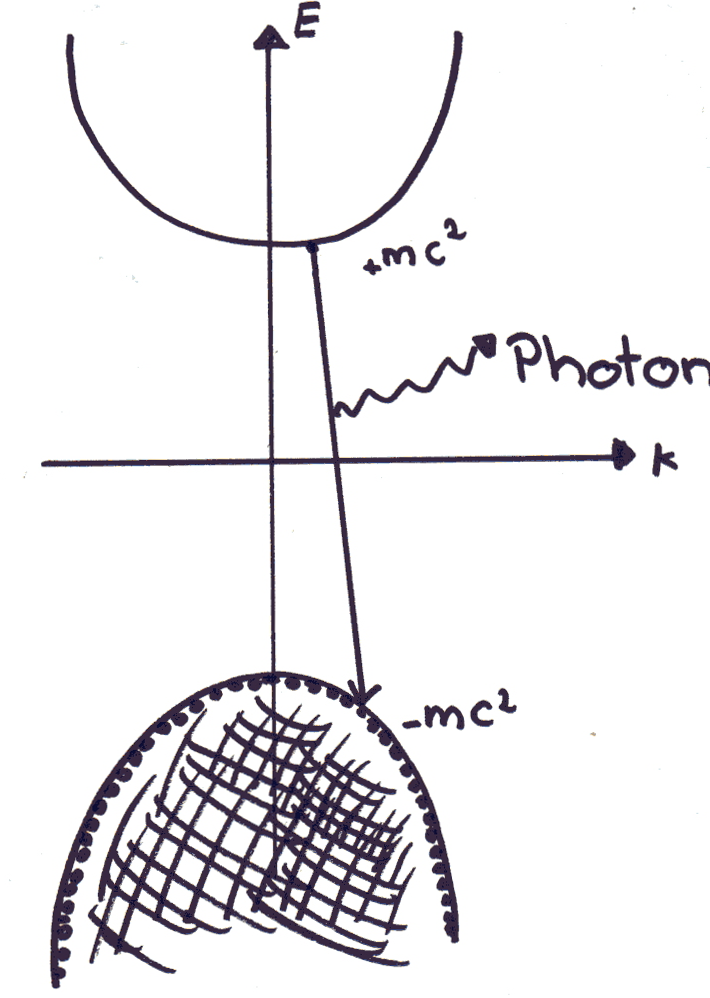
\includegraphics[scale=0.15]{Figs/Pim000114.png}
\end{center}
\end{wrapfigure}
\underline{Ausweg:} Dirac 1930\\
Alle Zustände negativer Energie sind besetzt. Wegen des Pauliverbots sind somit die Zustände negativer Energie für die Elektronen unerreichbar:\\

Der Vakuumzustand besteht aus einem See von unendlich vielen Teilchen negativer Energie, die alle Zustände besetzen.\\
\\
\underline{Anregung des Vakuums:}\\
Ein Elektron aus dem Diracsee wird in einem Zustand positiver Energie angeregt. Zurück bleibt ein \underline{Loch} im Diracsee mit folgenden Eigenschaften:
\begin{itemize}
\item Ladung:  $-q_e = e > 0$
\item Wellenfunktion des ursprünglichen Elektrons
\begin{eqnarray*} 
	v_s(p)e^{ipx} = v_s(p) e^{i(E_pt-\vec p\vec x)}
\end{eqnarray*} 
mit der Energie $-E_p>0$ und dem Impuls$-\vec p$. Ist der Zustand nicht besetzt, so ist der Energieunterschied größer 0. 
\item Spin:  $-s \frac \hbar 2$
\end{itemize}
\underline{Interpretation}\\
Das Loch verhält sich wie ein Teilchen mit der Energie $E$, Impuls $\vec p$, Ladung $+e$ und Spin $s\frac\hbar 2$.\\
$\Longrightarrow$ Antiteilchen (Positron)\\
Das Antiteilchen wurde experimentell nachgewiesen.

Probleme: 
\begin{itemize}
\item In der Diractheorie ist die Energie des Vakuums unendlich, und die Wechselwirkung zwischen den Teilchen wird vernachlässigt.
\item Die Dirac-Theorie dient der Beschreibung von Ein-Teilchen-Systemen. Im Dirac-See existieren aber unendlich viele Löcher. 
\item Es bleibt unklar, was für die Symmetriebrechung sorgt, die dazu führt, dass Elektronen und nicht Positronen unbesetzte Zustände besetzen. 
\end{itemize}

